%   File: frame_conventions.tex
% Author: Adam Leeper (with modifications by Paul Mitiguy)
%------------------------------------------------------------------------------
%\\[0.45pc]
\providecommand{\isolatedBuild}[1]{#1}% fallback definition lets this file build normally
\isolatedBuild{
  \documentclass[11pt,letterpaper]{book}
  %\documentclass[11pt,letterpaper]{book}

% aleeper: I think these are needed for Paul's macros?
\usepackage{epsfig}
\usepackage{epstopdf}

%\makeatletter
%\typeout{The import path is \import@path}
%\makeatother

\usepackage{import}

\subimport{./}{packagesMitiguy.sty}
\subimport{./}{macrosMitiguy.tex}
\subimport{./}{PageStylesMitiguy.tex}
\subimport{./}{macrosLeeper.tex}
 % Must be found via TEXINPUTS environment variable.
  \isolatedBuildHeader{Rotation Matrices}
                      {Frame Conventions}
}
%%%
%%%
%%%
Creating a flight simulator requires cooperation of engineers from multiple
disciplines (graphics and aeronautics) that have different frame conventions.
Many 3D graphics applications consider the ``world" frame to be defined as
shown by vector basis \basis{C}, where the ``ground" plane is defined by
\uvecx{c} and \uvecz{c}, with \uvecy{c} pointing opposite gravity.
Meanwhile, aeronautics uses a frame convention shown by vector basis \basis{D}
, where \uvecx{d} points north, \uvecy{d} points east, and \uvecz{d} points
in the direction of gravity (this convention is often called NED, for
``north-east-down").
For clarity, in the picture below the frames \basis{C} and
\basis{D} are ``aligned'' but use a different convention. Note \uvecz{c}
is ``out" of the page and \uvecx{d} is ``in."
%
\\[0.45pc]
To properly display aeronautics simulation data (computed and expressed in
\basis{D}) in the graphics engine, the data must be re-expressed using
the basis vectors of frame \basis{C}.
Form the rotation table \dircos{c}{d} relating \uvecxyz{c} to \uvecxyz{d}.
\\[0.0pc]
{ \footnotesize
  \textbf{Note:} The elements of the rotation table are numbers (no symbols).
}
\\[0.45pc]
\begin{minipage}[t]{0.5\linewidth}
  \vspace*{0pt}
  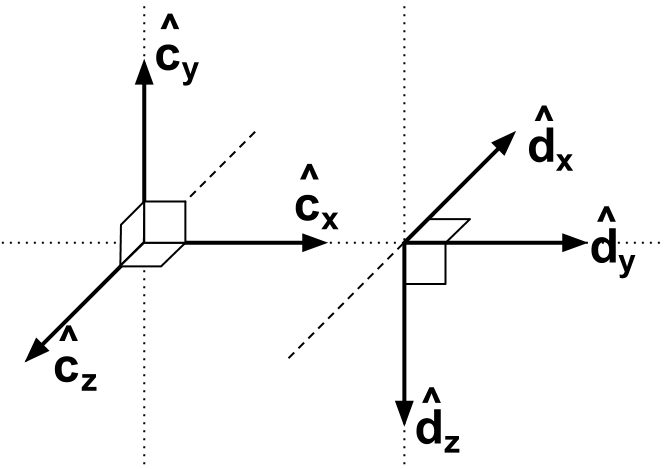
\includegraphics[height=5cm]{frame_conventions.png}
\end{minipage}
%\hfill
\begin{minipage}[t]{0.3\linewidth}
  \vspace*{0pt}
  \Solution {}{1.0\linewidth}{
    {  \Large
       \rotationTable{c}{d}
                     {~~ 0}{~ 1}{~~ 0}
                     {~~ 0}{~ 0}{ -1}
                     { -1} {~ 0}{~~ 0}
    }
  }
\end{minipage}
%
%
\isolatedBuildFooter
